
\section{Introdução}
Elevadores são dispositivos que estão presentes na maioria dos edifícios, sendo em muitos casos essenciais para o acesso das pessoas aos andares mais elevados. Um elevador, de forma genérica, possui sensores (botões de cada andar, sensor de posição) e atuadores (motor de subida/descida, motor das portas e luzes dos botões de andar).

Este projeto tem o objetivo de desenvolver um controlador de elevador com o Kit LPC1768, sendo que ele será responsável por gerenciar todos os aspectos da lógica de funcionamento do elevador.

\section{Objeto}
O produto tem o propósito de ser um controlador de elevador, recebendo requisições de usuários nos botões de cada andar e nos botões internos, e efetuando o controle dos atuadores (luzes de botões, motor de subida/descida e portas) conforme essas requisições. O elevador deve atender às demandas dos usuários, de forma eficiente.

\section{Domínio do problema}
Para o gerenciamento de um elevador, há aspectos importantes que devem ser observados com relação ao seu funcionamento.  O elevador possui limitações quando à sua aceleração máxima. Portanto, há um intervalo mínimo de tempo para ele conseguir parar quando recebe uma requisição de um usuário. Essas limitações estão expostas mas adinate nos requisitos não-funcionais.

Com relação à segurança, as portas somente devem ser abertas quando o elevador está parado em algum andar (posicionado dentro de uma faixa de segurança). Também, o elevador só deve mover-se com as portas fechadas.


% \subsection{Segurança}
% A segurança é um fator primordial, que, dentro do contexto deste projeto, envolve o gerenciamento correto dos motores do elevador (subida/descida e portas). Primeiramente, deve-se notar os fatores físicos 

\section{Contexto}

A Figura \ref{fig:diagrama_blocos} apresenta o diagrama de blocos com uma visão geral do sistema. Um computador executa continuamente uma simulação de elevador. O usuário interage diretamente com esta simulação através do mouse, pressionando botões (internos e externos) do elevador. O Kit LPC1768 faz o papel de controlador do elevador, gerenciando a lógica de movimentação e de abertura/fechamento de portas. O Kit e o computador comunicam-se via interface serial, sendo que o Kit controla o comportamento do elevador na simulação, e o computador envia ao Kit comandos de botões do usuário. 

\begin{figure}[h]
\begin{center}
    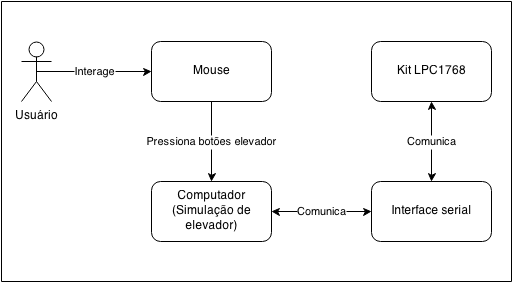
\includegraphics[width=0.8\columnwidth]{./figures/diagrama_blocos.png}
    \caption{Diagrama de blocos do sistema.}
    \label{fig:diagrama_blocos}
\end{center}
\end{figure}


\section{Interfaces}
[TODO: INSERIR FIGURA DO SIMULADOR]
[TODO: EXPLICAR INTERFACE SERIAL]


\section{Especificação funcional}



Os requisitos funcionais levantados para o \it{software} são:

\begin{enumerate}[label=RF \arabic*. , ref=\arabic*]
	\item O sistema deverá ligar a luz de um botão quando este for pressionado.
  \item O sistema deverá desligar a luz de um botão quando o elevador parar no andar correspondente ao botão.
  \item O sistema deverá abrir as portas quando o elevador parar em um andar.
  \item O sistema deverá impedir que as portas sejam abertas quando o elevador não estiver posicionado em um andar.
  \item O sistema deverá impedir que as portas sejam abertas quando o elevador estiver em movimento.
  \item O sistema deverá impedir que o elevador se movimente quando as portas estiverem abertas.
  \item O sistema deverá atender a requisições de mudança de andar, feitas através dos botões.
  \begin{enumerate}[label*=\arabic*.]
    \item O sistema deverá enfileirar as requisições de mudança de andar.
    \item O sistema deverá manter apenas uma requisição de cada andar na fila.
    \item O sistema deverá dar prioridade à requisições feitas com os botões internos.
    \item O sistema deverá dar prioridade às requisições dos andares mais altos feitas com botões externos de descida.
    \item O sistema deverá dar prioridade às requisições dos andares mais baixos feitas com botões externos de subida.
    \item O sistema deverá parar o elevador quando ele estiver passando por um andar que o botão interno correspondente tenha sido pressionado.
    \item O sistema deverá parar o elevador quando ele estiver passando por um andar que o botão externo tenha sido pressionado, se estiver indo na mesma direção que a requisição foi feita.
    \end{enumerate}
  \item O sistema deverá esperar no mínimo 5 segundos após as portas terem sido fechadas antes de fechar elas novamente.
  \item O sistema deverá esperar meio segundo após fechar as portas antes de deslocar o elevador.
  \item O sistema deverá esperar meio segundo após o elevador parar antes de abrir as portas.
  \item O sistema deverá esperar no mínimo 2 segundos para fechar a porta após um botão interno ser pressionado.
\end{enumerate}

\section{Especificação não-funcional}

Os requisitos não-funcionais levantados para o \it{software} são:

\begin{enumerate}[label=RNF \arabic*. , ref=\arabic*]
	\item O sistema deverá parar o elevador após chegar no andar em no máximo 40 milissegundos.
  \item O sistema deverá responder a uma requisição em no máximo 40 milissegundos.
  \item O sistema deverá acender a luz correspondente em no máximo 10 milissegundos após um botão ter sido pressionado.
\end{enumerate}








